% This example is meant to be compiled with lualatex or xelatex
% The theme itself also supports pdflatex
\PassOptionsToPackage{unicode}{hyperref}
\documentclass[aspectratio=1610, 9pt]{beamer}

% Load packages you need here
\usepackage{polyglossia}
\setmainlanguage{german}

\usepackage{csquotes}
    

\usepackage{amsmath}
\usepackage{amssymb}
\usepackage{mathtools}

\usepackage{hyperref}
\usepackage{bookmark}

% load the theme after all packages

\usetheme[
  showtotalframes, % show total number of frames in the footline
]{tudo}

% Put settings here, like
\unimathsetup{
  math-style=ISO,
  bold-style=ISO,
  nabla=upright,
  partial=upright,
  mathrm=sym,
}

%Titel:
\title{Neutrinodetektoren und Upgrades}
%Autor
\author[N.Breer]{Nils Breer}
%Lehrstuhl/Fakultät
\institute{Fakultät Physik}
%Titelgrafik muss ich einfueren!!!
%\titlegraphic{\includegraphics[width=0.3\textwidth]{content/Bilder/interferenz.jpg}}
\date{13.12.2019}

\begin{document}
\maketitle

\begin{frame}\frametitle{Agenda}
  \begin{itemize}
    \item IceCube + Upgrade
    \item KM3NET
    \item ANTARES
    \item BAIKAL + GVD
    \item STRAW + P-ONE
  \end{itemize}
\end{frame}

\begin{frame}\frametitle{IceCube Aufbau}
  \begin{columns}
  \begin{column}[c]{0.45\textwidth}
    \begin{itemize}
      \item square-kilometer detektor am geographischen S\"udpol
      \item 2500m dicke Eisschicht
      \item hexagonales gitter mit "strings"
      \item 5160 DOMs, 86 strings
      \item spacing: 17m vertikal, 125m horizontal
    \end{itemize}
  \end{column}
  \begin{column}[c]{0.45\textwidth}
    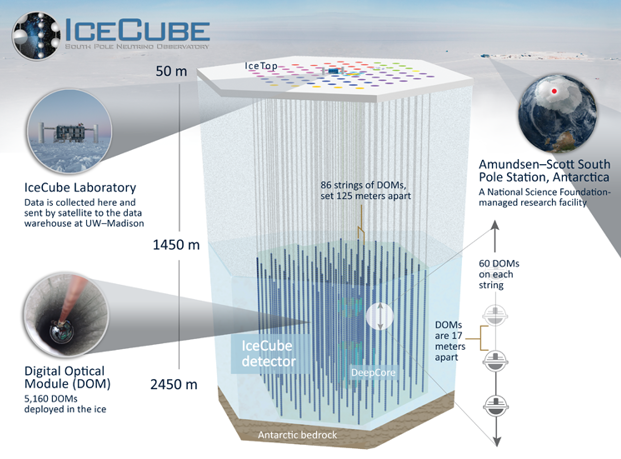
\includegraphics{images/icecube.png}
  \end{column}
  \end{columns}
\end{frame}

\begin{frame}\frametitle{IceTop}
  \begin{itemize}
    \item 81 Stationen oberhalb der Strings
    \item Dient als Veto und zur Kallibration
    \item Detektion von Teilchenschauern in der Atmosphere \"uber IceCube
    \item Sensitiv auf Energiebereich 300 TeV - 1 EeV
    \item Messung der Strahlkomposition
  \end{itemize}
\end{frame}

\begin{frame}\frametitle{DeepCore}
  \begin{itemize}
    \item kompaktes hexagonales Raster im inneren von IceCube
    \item senkt die Schwellenenergie auf ca. 10 GeV
    \item Studieren der Neutrinooszillation
  \end{itemize}
\end{frame}

\begin{frame}\frametitle{Wie funktioniert eine PMT?}
  \begin{columns}
    \begin{column}[c]{0.45\textwidth}
      \begin{itemize}
      \item PMT $\to$ Photomultiplier Tube
      \item $\gamma$ trifft auf Photokathode $\to$ Photoeffekt
      \item Prim\"arelektron l\"ost an jeder Dynode neue $e^{-}$ aus
      \item Abflie\ss en aller $e^{-}$ \"uber Widerstand $\to$ Spannungsabfall $\to$ Signal
      \item Verst\"arkung $\symup{\delta}$ $\approx$ $4^{10}$ \,-\, $6^{10}$
      \end{itemize}
    \end{column}
    \begin{column}[c]{0.45\textwidth}
      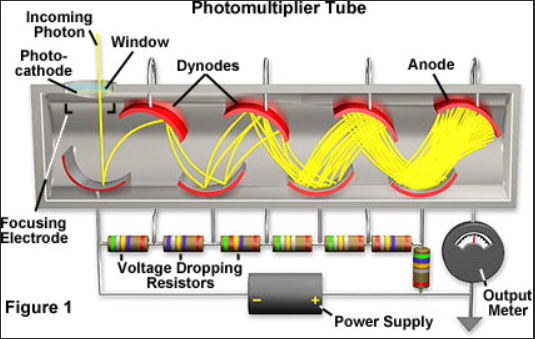
\includegraphics{images/pmt.png}
    \end{column}
  \end{columns}
\end{frame}

\begin{frame}\frametitle{Wie detektiert man Neutrinos eigentlich?}
  \begin{columns}
    \begin{column}[c]{0.45\textwidth}
      \begin{itemize}
      \item $\nu_{l}$ wechselwirkt mit Eis $\to$ geladenes Lepton
      \item Cherenkov Licht des geladenen Teilchens $\to$ detektion durch PMT's
      \item speichern des timestamps von Signal des PMT
      \item Richtung und Geschwindigkeit des Neutrinos
      \end{itemize}
    \end{column}
    \begin{column}[c]{0.45\textwidth}
      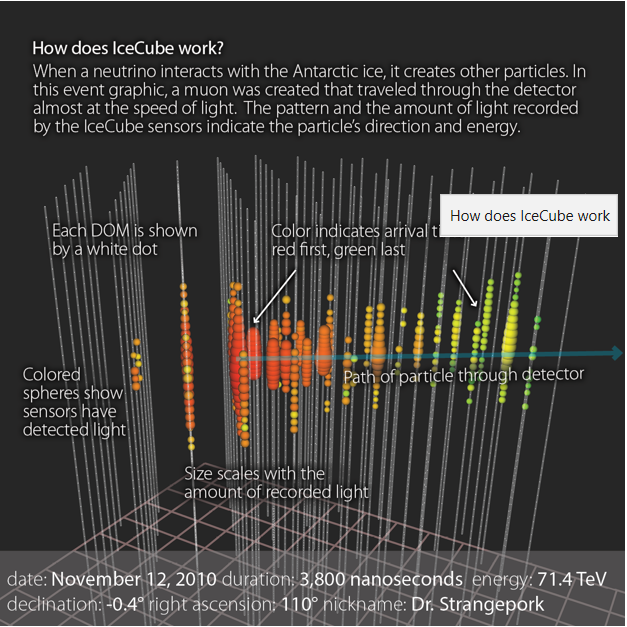
\includegraphics{images/signal_test.png}
    \end{column}
  \end{columns}
\end{frame}

\begin{frame}\frametitle{IceCube Upgrade}
  \begin{itemize}
    \item 
  \end{itemize}
\end{frame}

\begin{frame}\frametitle{KM3NET}
  \begin{itemize}
    \item 
  \end{itemize}
\end{frame}

\begin{frame}\frametitle{ANTARES}
  \begin{itemize}
    \item 
  \end{itemize}
\end{frame}

\begin{frame}\frametitle{BAIKAL + GVD}
  \begin{itemize}
    \item 
  \end{itemize}
\end{frame}

\begin{frame}\frametitle{GVD}
  \begin{itemize}
    \item 
  \end{itemize}
\end{frame}

\begin{frame}\frametitle{STRAW + P-ONE}
  \begin{itemize}
    \item 
  \end{itemize}
\end{frame}

\begin{frame}\frametitle{P-ONE}
  \begin{itemize}
    \item 
  \end{itemize}
\end{frame}

\begin{frame}\frametitle{Quellen}
\url{https://icecube.wisc.edu/science/icecube/detector} \\
\url{https://micro.magnet.fsu.edu/primer/digitalimaging/concepts/photomultipliers.html} \\

\end{frame}

\end{document}